\section{Results and discussion}

\subsection{Volume recovery with fewer measurements}

\begin{figure}[htbp]
\centering
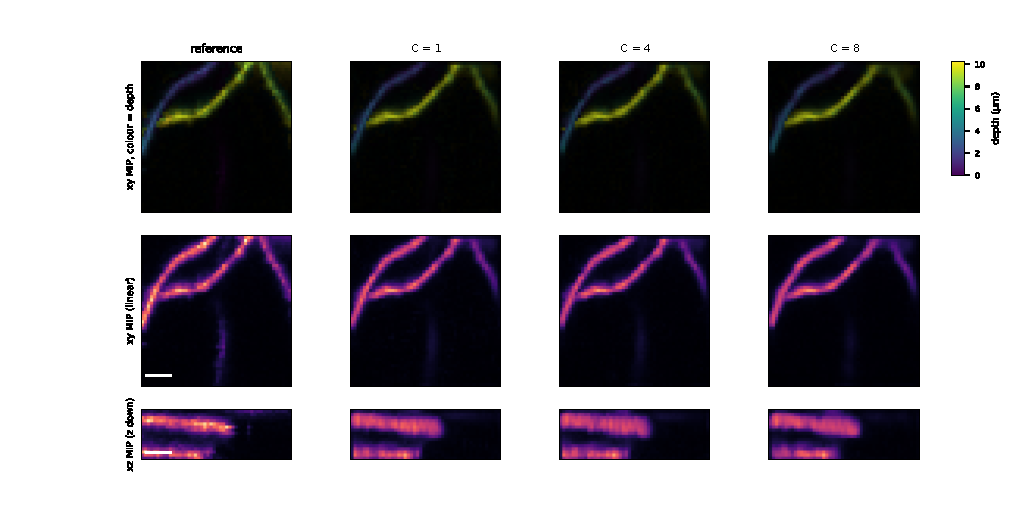
\includegraphics[width=\linewidth]{figures/neurons.pdf}
\caption{Mouse pyramidal neuron volume recovery at compression factors C=1, 4 and 8
(reference-selected subvolume 384, separate from the test set).
Rows: depth-coloured and intensity lateral maximum-intensity projections (MIPs), then xz MIPs.
Depth colour indicates the brightest voxel along each column.
All panels share intensity limits [0,0.880] and physical aspect ratio;
bars: 5 micrometres at the assigned simulation scale.}
\label{fig:neuronal}
\end{figure}


Angle-scanned phase illumination enables volume recovery from fewer scalar measurements than reconstructed voxel values. In the representative reconstruction shown in Figure 3, dominant dendritic structures and their depth ordering remain recognisable even at eight-fold compression. The depth-oriented views also reveal axial thickening, and a faint vertical neurite is largely lost even without compression. The retained large-scale structure therefore coexists with incomplete recovery of finer features.

Table 2 summarises performance across the eight-subvolume test set. At \(C=8\), mean depth error increases from \(0.497\) to \(0.626\,\mu\mathrm m\), while foreground SSIM decreases from 0.679 to 0.588. The paired depth increase is \(0.129\pm0.032\,\mu\mathrm m\), with a PSNR decrease of \(0.91\pm0.45\,\mathrm{dB}\). At \(C=4\), the corresponding changes are smaller: \(0.053\pm0.016\,\mu\mathrm m\) in depth error and \(0.45\pm0.35\,\mathrm{dB}\) in PSNR. Depth error increases in every test subvolume at both compression levels, with four-fold increases ranging from \(0.025\) to \(0.076\,\mu\mathrm m\). These paired comparisons distinguish compression costs from variation between specimen structures.

\begin{table}[htbp]
\centering\caption{Eight-subvolume test set. Mean and sample SD across subset-averaged subvolumes; paired changes use each subvolume's own uncompressed acquisition.}
\begin{tabular}{@{}>{\raggedright\arraybackslash}p{0.176000\linewidth}@{\hspace{0.03\linewidth}}>{\raggedright\arraybackslash}p{0.176000\linewidth}@{\hspace{0.03\linewidth}}>{\raggedright\arraybackslash}p{0.176000\linewidth}@{\hspace{0.03\linewidth}}>{\raggedright\arraybackslash}p{0.176000\linewidth}@{\hspace{0.03\linewidth}}>{\raggedright\arraybackslash}p{0.176000\linewidth}@{}}\toprule
Compression \(C\) & Depth error (\(\mu\mathrm m\)) & Foreground SSIM & Paired depth change (\(\mu\mathrm m\)) & Paired SSIM change \\
\midrule
1 & \(0.497\pm0.183\) & \(0.679\pm0.238\) & 0 & 0 \\
4 & \(0.550\pm0.170\) & \(0.652\pm0.252\) & \(+0.053\pm0.016\) & \(-0.027\pm0.025\) \\
8 & \(0.626\pm0.207\) & \(0.588\pm0.273\) & \(+0.129\pm0.032\) & \(-0.091\pm0.040\) \\
\bottomrule\end{tabular}
\end{table}

Recovery quality varies across specimen structures. The two dense subvolumes, with approximately 30--34\% occupancy, have uncompressed foreground SSIM of 0.44--0.47; the near-empty subvolume has an unstable foreground metric because of its limited support. The separate ablation example, subvolume 0, has depth errors of \(0.177\), \(0.231\) and \(0.276\,\mu\mathrm m\) at \(C=1,4,8\). The test set captures variability beyond these separate examples.

Synthetic beads separate detection accuracy from depth placement (Figure 4). The detection Jaccard index remains 1.00 at \(C=1,4,8\), but mean depth error increases from \(0.183\) to \(0.282\) and \(0.544\,\mu\mathrm m\), respectively. The corresponding mirror-to-true-depth energy ratios are 0.011, 0.012 and 0.035. Thus all beads remain detectable under compression, while their depth placement becomes less precise and mirror-depth leakage increases.


\begin{figure}[htbp]
\centering
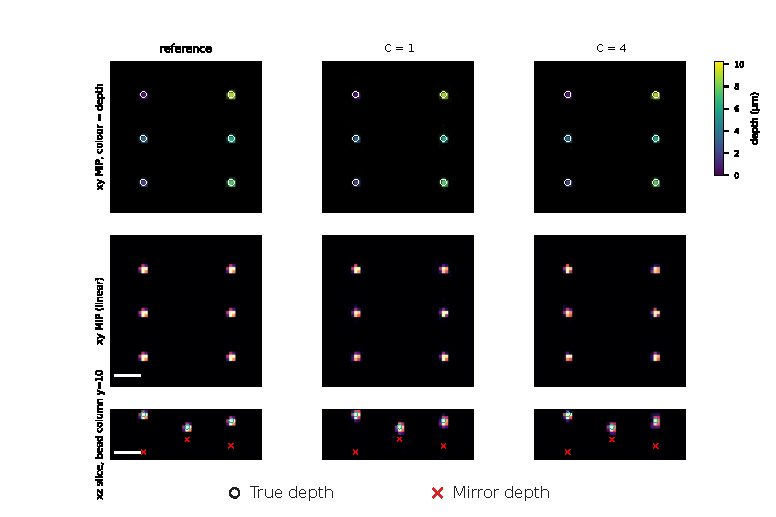
\includegraphics[width=0.96\linewidth,height=0.43\textheight,keepaspectratio]{figures/beads.pdf}
\caption{Synthetic bead recovery at C=1 and C=4.
Rows: depth-coloured and intensity lateral MIPs, then an xz slice at lateral index 10.
Circles mark true positions and crosses mirror positions.
All panels share intensity limits [0,1] and physical aspect ratio;
bars: 5 micrometres at the assigned simulation scale.}
\label{fig:beads}
\end{figure}

\subsection{Ablation studies}

The following ablations examine how the measurement model, illumination encoding and reconstruction prior contribute to recovery. We then consider angular coverage and the trade-off at stronger compression.

\subsubsection{Model mismatch and voxel integration}

\begin{figure}[htbp]
\centering
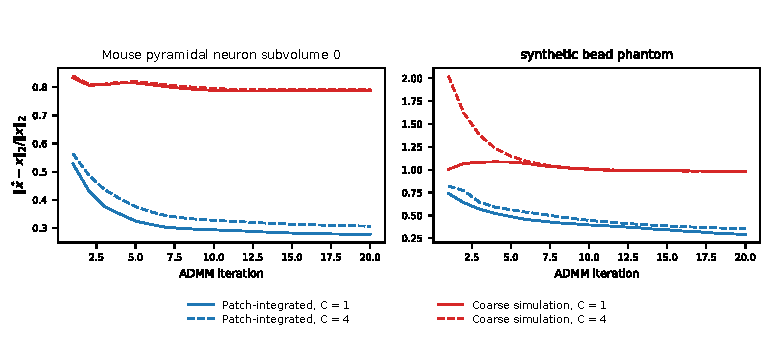
\includegraphics[width=\linewidth,height=0.28\textheight,keepaspectratio]{figures/model_mismatch.pdf}
\caption{Effect of voxel modelling on reconstruction error.
Patch-integrated and coarse-simulation curves average three noise realisations;
solid/dashed lines denote C=1/C=4.}
\label{fig:mismatch}
\end{figure}


We compare voxel-integrated fine-grid modelling with direct optical simulation at the \(0.64\,\mu\mathrm m\) reconstruction spacing. Both reconstruct identical fine-grid measurements with the same iteration budget and separately validated parameters.

For subvolume 0, patch integration reduces the noise-free relative forward discrepancy from 25.7\% to 1.07\% and improves reconstruction (Table 3, Figure 5). The difference has a physical basis: the high-NA field requires lateral sampling no coarser than \(\lambda/(2\mathrm{NA})\simeq0.33\,\mu\mathrm m\), so direct simulation at \(0.64\,\mu\mathrm m\) cannot represent its full spatial bandwidth.

\begin{table}[htbp]
\centering\caption{Voxel-model ablation: mouse pyramidal neuron subvolume 0, uncompressed acquisition, mean over three noise realisations. Depth errors are in micrometres, not voxel planes.}
\begin{tabular}{@{}>{\raggedright\arraybackslash}p{0.227500\linewidth}@{\hspace{0.03\linewidth}}>{\raggedright\arraybackslash}p{0.227500\linewidth}@{\hspace{0.03\linewidth}}>{\raggedright\arraybackslash}p{0.227500\linewidth}@{\hspace{0.03\linewidth}}>{\raggedright\arraybackslash}p{0.227500\linewidth}@{}}\toprule
Operator & Depth error (\(\mu\mathrm m\)) & Foreground SSIM & PSNR (dB) \\
\midrule
Patch-integrated & 0.177 & 0.913 & 37.22 \\
Coarse optical simulation & 1.859 & 0.356 & 28.12 \\
\bottomrule\end{tabular}
\end{table}

The advantage persists at \(C=4\), with depth errors of \(0.236\,\mu\mathrm m\) for patch integration and \(1.867\,\mu\mathrm m\) for coarse simulation. Accurate optical modelling therefore remains important under measurement compression.

\subsubsection{In-focus DMD baseline}

A digital micromirror device (DMD) generates illumination patterns by amplitude modulation, as in DEEP and DEEP². We compare this alternative with the phase encoder to test whether amplitude-pattern variation provides the depth information required for volumetric recovery.

For ideal scalar propagation through an aberration-free symmetric relay, a real-valued focal-plane field \(U\) gives conjugate fields at opposite defocus and hence equal excitation intensities:
\[
U(\mathbf r,-\Delta z)=U(\mathbf r,+\Delta z)^*,\qquad
I(\mathbf r,z_{\mathrm{focus}}-\Delta z)
=I(\mathbf r,z_{\mathrm{focus}}+\Delta z).
\]
A defocused phase encoder supplies a complex field at the relay image plane, removing this symmetry constraint. The vectorial simulations show the same contrast between the two geometries.

To distinguish mirror ambiguity from local depth sensitivity, we use the point-emitter response \(\mathbf a(z)\) at fixed lateral position. With unknown brightness \(b\) and Gaussian noise scale \(\sigma\), the axial information and mirror separation are
\[
\begin{aligned}
\mathcal I_z&=\frac{b^2}{\sigma^2}
\left(\|\partial_z\mathbf a\|_2^2-
\frac{(\mathbf a^\top\partial_z\mathbf a)^2}{\|\mathbf a\|_2^2}\right),
&\sigma_z&\geq\mathcal I_z^{-1/2},\\
d'&=\min_c\frac{\|b\mathbf a(z)-c\mathbf a(z_m)\|_2}{\sigma},
&z_m&=2z_{\mathrm{focus}}-z .
\end{aligned}
\tag{9}
\]
Here \(c\) fits the brightness at the mirror depth. Medians cover 144 lateral positions and interior depth planes, with \(0.32\,\mu\mathrm m\) central differences and the focus excluded from mirror comparisons. The diagnostic uses \(b=1\), \(q=25\); recovery uses \(q=15\).

The DMD and phase plate have similar local axial bounds, \(0.02183\) and \(0.01885\,\mu\mathrm m\), but markedly different mirror separation: \(d'=0.0379\) and 44.76, respectively. Local depth sensitivity therefore does not guarantee separation of mirror-related positions; these bounds are not optical-resolution measurements.

With the same pretrained denoiser and solver and separately validated parameters, uncompressed neuronal reconstruction gives depth errors of \(1.775\,\mu\mathrm m\) for the DMD and \(0.177\,\mu\mathrm m\) for the phase plate. The DMD error approaches the empty-volume value of \(1.88\,\mu\mathrm m\), showing that the prior cannot replace depth-distinguishing measurements. Bead mirror energy ratios of 1.007 and 0.011 confirm the contrast. This comparison concerns the evaluated in-focus geometry and uses each encoder's relative-noise scale, not matched calibrated photon counts.

\subsubsection{Effect of slice fusion}

To assess the reconstruction prior, we compare fused and individual slice orientations on uncompressed subvolume 0. Three-orientation fusion reaches 37.22 dB PSNR, compared with 36.26--36.81 dB for individual orientations and 33.99 dB for sparsity alone. The best single orientation, \(xy\), has slightly lower depth error than fusion (\(0.163\) versus \(0.177\,\mu\mathrm m\)); fusion improves intensity fidelity, not every metric. Removing sparsity from the fused configuration leaves PSNR at 37.22 dB, indicating no additional PSNR benefit at the evaluated sparsity weight.

\subsubsection{Angular coverage and measurement allocation}

At a fixed pattern count, our preliminary scan-design experiments found lower maximum pairwise output-field correlation with balanced azimuth/elevation allocations than with strongly unbalanced grids. Detector-size experiments also showed that allocating more measurements to illumination diversity could improve recovery. These findings motivate balanced angular coverage and the measurement-count evaluation.

Equation (1a) explains why equal angular increments need not give equal phase-gradient changes. With \(\rho=|\cos\theta|\), direction-space separations are \(2\rho|\sin(\Delta\alpha/2)|\) for azimuth steps and \(|\cos(\theta+\Delta\theta)-\cos\theta|\) for elevation steps. Since \(M=Pk\), fewer detector samples per image permit more illumination directions at a fixed measurement count. We fix the detector, evaluate \(k=256,64,32\), and draw compressed subsets across the full angular grid.

\subsubsection{Higher compression factors}

Extending the compression test on subvolume 0 gives foreground SSIM of 0.832 and 0.761 at \(C=16,32\), compared with 0.913 at \(C=1\). Depth errors rise to \(0.354\) and \(0.443\,\mu\mathrm m\). These exploratory results show the growing trade-off; the main assessment remains \(C=1,4,8\) across eight subvolumes.

\subsection{Discussion and limitations}

The results connect depth encoding, voxel-integrated modelling and multi-slice recovery. The illumination supplies depth-distinguishing measurements, the integrated model represents their dependence on the volume, and slice priors regularise the inverse problem. Representative reconstructions retain dominant dendritic structures at eight-fold compression, while the test set quantifies the fidelity trade-off. Recovery from angular subsets is consistent with redundancy among correlated illumination patterns; independent patterns are not required or assumed.

The acquisition builds on illumination-coded volumetric microscopy. Speckle microscopy already recovers depth from lateral scans, including in nonsaturated fluorescence \cite{pascucci2019}. Within this family, our study evaluates angle variation at a fixed phase encoder together with voxel-integrated modelling and multi-slice reconstruction. The mismatch ablation explains why retaining fine optical responses and integrating over the reconstruction basis improves recovery, while the analytical factorisation makes that model practical to construct.

This study is numerical. The optical model assumes linear fluorescence in a homogeneous, negligible-scattering medium and equal excitation and detection wavelengths. Its additive Gaussian noise is a relative-noise model rather than calibrated photon noise, and reconstructions use a fixed iteration budget. Sampling intervals, centroid errors and local point-emitter bounds should not be interpreted as optical resolution.

Experimental implementation would require calibrated illumination and detection responses and controlled alignment. A phase-only SLM could implement the encoder, while learned phase profiles may improve recovery at stronger compression. Within PnP, a task-specific three-dimensional denoiser could exploit volumetric structure more directly and potentially support stronger compression when sufficient training data and computational resources are available. These learned extensions remain future directions.
